\documentclass[a4paper,titlepage]{book}
\usepackage{frontespizio}
\usepackage[italian]{babel}
\usepackage[utf8]{inputenc}
\usepackage{usecases}

\usepackage{tikz}
\usetikzlibrary{arrows,shadows} % for pgf-umlsd
\usepackage[underline=true,rounded corners=false]{pgf-umlsd}

\usepackage{enumitem}
\setitemize{noitemsep,topsep=0pt,parsep=0pt,partopsep=0pt}

\usepackage[a4paper, total={6in, 9in}]{geometry}

\begin{document}
\begin{frontespizio}
\Universita{Verona}
\Facolta{Scienze Matematiche, Fisiche e Naturali}
\Corso[Laurea]{Informatica}
\Titoletto{Tesi di laurea}
\Titolo{Sistema domotico a basso costo\\pilotato con protocollo Modbus}
\Candidato[VR359169]{Enrico Giordano}
\Relatore{Prof. Graziano Pravadelli}
\Annoaccademico{2013-2014}
\end{frontespizio}




%%%%%%%%%%%%%%%%%%%%%%%%%%%%%%%%%%%%%%%%%%%%%%%%%%%%%%%%%%%%%%%%%%%%%%%%%%%%%%%%%%%%%%%%%%%%%%%%%%%%%%%%%%%%%%%%%%%%%%%%%%%%%%%%%%%%%%%%%
%%%%%%%%%%%%%%%%%%%%%%%%%%%%%%%%%%%%%%%%%%%%%%%%%%%%%%%%%%%%%%%%%%%%%%%%%%%%%%%%%%%%%%%%%%%%%%%%%%%%%%%%%%%%%%%%%%%%%%%%%%%%%%%%%%%%%%%%%
%%%%%%%%%%%%%%%%%%%%%%%%%%%%%%%%%%%%%%%%%%%%%%%%%%%%%%%%%%%%%%%%%%%%%%%%%%%%%%%%%%%%%%%%%%%%%%%%%%%%%%%%%%%%%%%%%%%%%%%%%%%%%%%%%%%%%%%%%
%%%%%%%%%%%%%%%%%%%%%%%%%%%%%%%%%%%%%%%%%%%%%%%%%%%%%%%%%%%%%%%%%%%%%%%%%%%%%%%%%%%%%%%%%%%%%%%%%%%%%%%%%%%%%%%%%%%%%%%%%%%%%%%%%%%%%%%%%

\chapter*{Introduzione}
La domotica è una scienza interdisciplinare che si occupa di creare oggetti utili a migliorare la qualità della vita nella casa e più in generale negli ambienti abitati, favorendo la serenità e facendo risparmiare tempo (e soprattutto denaro) per la gestione le faccende domestiche.
 
Con l'avanzare della tecnologia, vengono utilizzati strumenti sempre più complessi, favorendo un sistema \textit{``user friendly''} ma costoso, che dal punto di vista finanziario non è accessibile per la maggior parte delle famiglie. Un fattore che avvicina gli sviluppatori a queste tecnologie è la semplicità di progettazione: più avanzata è l'architettura, quindi definibile \textit{``general purpoise''}, più è facile sviluppare nuovo software e mantenerlo nel tempo. Queste architetture però non sono dedicate esclusivamente all'ambito di utilizzo; questo è un fattore che impreziosisce tutto il progetto nel complesso e di conseguenza fa aumentare il prezzo di mercato del progetto stesso.

La soluzione a questo problema è progettare un sistema dedicato, \textit{``embedded''}, in grado di occuparsi esclusivamente di alcuni compiti e ottimizzato sia nei costi che nell'esecuzione delle operazioni specifiche. Questo può essere un limite per vari fattori, ossia difficoltà di sviluppo, difficoltà di scelta della componentistica, ottimizzazione di risorse e codice, però offre il vantaggio di essere un progetto a basso costo dal punto di vista sia hardware che software, in quanto si propone qualcosa di più semplice ma efficace.

~

Questo progetto rappresenta un piccolo sistema domotico con cui si controllano le luci di una casa e i vari sensori che monitorano le stanze, utilizzando un pannello di controllo Master che comunica con le diverse periferiche slave tramite protocollo Modbus.


\tableofcontents


%%%%%%%%%%%%%%%%%%%%%%%%%%%%%%%%%%%%%%%%%%%%%%%%%%%%%%%%%%%%%%%%%%%%%%%%%%%%%%%%%%%%%%%%%%%%%%%%%%%%%%%%%%%%%%%%%%%%%%%%%%%%%%%%%%%%%%%%%
%%%%%%%%%%%%%%%%%%%%%%%%%%%%%%%%%%%%%%%%%%%%%%%%%%%%%%%%%%%%%%%%%%%%%%%%%%%%%%%%%%%%%%%%%%%%%%%%%%%%%%%%%%%%%%%%%%%%%%%%%%%%%%%%%%%%%%%%%
%%%%%%%%%%%%%%%%%%%%%%%%%%%%%%%%%%%%%%%%%%%%%%%%%%%%%%%%%%%%%%%%%%%%%%%%%%%%%%%%%%%%%%%%%%%%%%%%%%%%%%%%%%%%%%%%%%%%%%%%%%%%%%%%%%%%%%%%%
%%%%%%%%%%%%%%%%%%%%%%%%%%%%%%%%%%%%%%%%%%%%%%%%%%%%%%%%%%%%%%%%%%%%%%%%%%%%%%%%%%%%%%%%%%%%%%%%%%%%%%%%%%%%%%%%%%%%%%%%%%%%%%%%%%%%%%%%%


\chapter{Il progetto}

Il progetto consiste in un sistema domotico utilizzabile da un qualunque utente (quindi non esperto di informatica) mediante interfaccia grafica intuitiva ed essenziale. È composto essenzialmente da diversi dispositivi che devono comunicare tra loro in base alle scelte che l'utente attua navigando nell'interfaccia. Deve esserci quindi un dispositivo centrale che trasforma gli ordini ad alto livello dell'utente in istruzioni per gli altri dispositivi.

~

L'utente è in grado di eseguire operazioni di controllo della casa, tramite sensori presenti nelle stanze, e di interazione con oggetti fisici, ossia luci e motori per aprire o chiudere porte. Tutto ciò deve risultare semplice e intuitivo all'utente, quindi la comunicazione e il controllo devono essere gestiti interamente dai dispositivi, mentre l'utente deve essere solo in grado di fare la scelta tramite appositi pulsanti che compaiono nell'interfaccia. È presente quindi un menù in base al quale si sceglie il tipo di comando da eseguire e, in base alla scelta principale si viene indirizzati alla schermata apposita.

~

Ogni sintomo di guasto può essere diagnosticato tramite un'interfaccia particolare, chiamata di \textit{debug}, che permette ad un tecnico di interfacciarsi con il sistema e capire il tipo di guasto (se è un guasto delle periferiche, se dei dispositivi, ecc ...). Anche l'utente può interfacciarsi con questa schermata seguendo le istruzioni del manuale; essendo basata la comunicazione su protocollo standard, è possibile imparare e comprendere i comandi per potersi interfacciare direttamente con i dispositivi fisici.  

~

Per questioni di prestazioni, di modularità e di costi, è necessario che ci sia un dispositivo centrale (che mostra l'interfaccia grafica) in grado di comunicare con protocollo standard con gli altri disposivi. Nell'architettura deve quindi esserci un dispositivo di tipo ''Master`` che comunica con dispositivi di tipo ''Slave`` in modo da inviargli i comandi scelti dall'utente tramite GUI. Il motivo di questa scelta è dovuto essenzialmente a due fattori:

\begin{itemize}[noitemsep,topsep=10pt,parsep=23pt,partopsep=0pt]
\item se ci fosse un dispositivo che si occupa di tutte le operazioni del sistema, le prestazioni sarebbero nettamente inferiori rispetto a ciò che ci si aspetta, altrimenti bisogna utilizzare un sistema più potente e quindi più costoso;

\item più dispositivi possono essere posizionati in posti diversi in un'abitazione: in questo caso si assicura che ogni dispositivo sia efficace nel controllo di una sola stanza;

\item per questioni estetiche, avere troppi fili in una casa può essere ''brutto`` e scomodo;

\item tirare troppi fili da un unico dispositivo crea diversi problemi, sia di modularità (\textit{da dove viene questo filo?}) sia di disponibilità da parte del dispositivo centrale (\textit{quanti fili posso controllare con il dispositivo?}) piuttosto che di diagnostica (\textit{questo filo cosa controlla?}).


\end{itemize}

~

A livello di costi, avere un dispositivo molto potente è molto più costoso di avere più dispositivi dedicati che, se ottimizzati, costano molto poco.
Per questo progetto verranno utilizzate delle demoboard, quindi oggetti non ottimizzati e progettati per avere un ambiente di sviluppo facile da configurare; si vedrà alla fine che ottimizzando le risorse i costi generali saranno molto ridotti.

~

Infine il sistema è stato progettato per essere espandibile: seguendo questo documento, è possibile creare un nuovo dispositivo in grado di interfacciarsi con il dispositivo ''Master``, in modo da controllare più periferiche e quindi più stanze. Inoltre, poichè la comunicazione utilizzata è standard, è possibile controllare anche dispositivi di diversa natura utilizzando la schermata di \textit{debug}.

~

I sensori utilizzati devono generare un segnale comprensibile ai dispositivi che li devono controllare: devono essere quindi convertitori di condizioni ambientali analogici o digitali, il cui tasso di discretizzazione non deve superare i 16 bit. Questo vincolo è imposto per questioni economiche e di sistema, si vedrà in seguito che l'architettura scelta e il protocollo utilizzato gestiscono al meglio dati a 16 bit.

~

Le luci da pilotare devono essere a LED, per diversi fattori:

\begin{itemize}[noitemsep,topsep=10pt,parsep=23pt,partopsep=0pt]

\item sono la nuova tecnologia di luci;

\item il voltaggio richiesto è adeguato al sistema, in questo modo si risparmia scegliendo un unico alimentatore di potenza adeguata;

\item risultano essere un investimento, in quanto costano di più rispetto alle normali lampadine, però durano per molto più tempo, quindi si ha solo la spesa aggiuntiva iniziale, ma risulta meno costosa come tecnologia perché non ha ricambi (se non in casi eccezionali).

\end{itemize}

%%%%%%%%%%%%%%%%%%%%%%%%%%%%%%%%%%%%%%%%%%%%%%%%%%%%%%%%%%%%%%%%%%%%%%%%%%%%%%%%%%%%%%%%%%%%%%%%%%%%%%%%%%%%%%%%%%%%%%%%%%%%%%%%%%%%%%%%%
%%%%%%%%%%%%%%%%%%%%%%%%%%%%%%%%%%%%%%%%%%%%%%%%%%%%%%%%%%%%%%%%%%%%%%%%%%%%%%%%%%%%%%%%%%%%%%%%%%%%%%%%%%%%%%%%%%%%%%%%%%%%%%%%%%%%%%%%%
%%%%%%%%%%%%%%%%%%%%%%%%%%%%%%%%%%%%%%%%%%%%%%%%%%%%%%%%%%%%%%%%%%%%%%%%%%%%%%%%%%%%%%%%%%%%%%%%%%%%%%%%%%%%%%%%%%%%%%%%%%%%%%%%%%%%%%%%%
%%%%%%%%%%%%%%%%%%%%%%%%%%%%%%%%%%%%%%%%%%%%%%%%%%%%%%%%%%%%%%%%%%%%%%%%%%%%%%%%%%%%%%%%%%%%%%%%%%%%%%%%%%%%%%%%%%%%%%%%%%%%%%%%%%%%%%%%%



\chapter{Architettura Hardware}

È stato deciso di attuare maggiore modularità possibile, in modo da poter descrivere nel dettaglio ogni componente e la sua funzione, ma soprattutto per potenziare l'intero sistema nel corso del tempo. 
Per la realizzazione di questo sistema, sono state scelte 3 tecnologie differenti, associate ognuna ad un compito diverso e con software specifico.



\section{LPC1788}
Questo è un microprocessore ARM di famiglia Cortex-M3 utilizzato come dispositivo Master che controlla tutti gli altri dispositivi. È un processore a 32 bit, quindi in grado di avere $2^{32}$ spazi di indirizzamento. Le sue periferiche principali sono: GPIO, I2C, UART, USB, EMAC, Ethernet, AUX Stereo, INPUT Mono, PWM a 32 bit, ADC, DAC. Può essere alimentato con $3,3 \sim 5 V$ e assorbe $200 mA$. Possiede $512KB$ di memoria FLASH, $96KB$ di memoria SRAM, $8MB$ di SDRAM (esterna), $1KB$ di memoria sicura EEPROM (esterna) per poter resettare guasti irreparabili (perdita di BIOS, anomalie su codice, ecc...). La grande quantità di memoria FLASH permette di sviluppare un software molto esteso. Poiché al suo interno è stata integrata una GPU, offre maggiori prestazioni grafiche, quindi è stato utilizzato per presentare l'interfaccia grafica per poter interagire con tutto il sistema. Di questo processore sono state utilizate queste periferiche:

\begin{itemize}[noitemsep,topsep=10pt,parsep=23pt,partopsep=0pt]

\item \textbf{GPU} per gestione di LCD TouchScreen VGA 640x480 5.7", utilizzato quindi per mostrare l'interfaccia grafica;
\item \textbf{RS232} per la comunicazione seriale tra dispositivi;
\item \textbf{Timer} per la gestione asincrona del tempo rispetto al ciclo di clock;
\item \textbf{Cicalina} per riprodurre suoni di avviso o di errore.

\end{itemize}

Il costo associato quindi a questo componente è:

\begin{tabular}{|l  r|}
\hline
\multicolumn{1}{|c|}{\textbf {oggetto}} & \multicolumn{1}{c|}{\textbf {Costo (in Euro)}} \\
\hline

processore 				& 18 \\
convertitore segnali TTL - RS232 	&  2  \\
LCD 					& 20 \\
\hline
\hline

\textit{\textbf{Totale:}}		& \textbf{40} \\

\hline
\end{tabular}
 

\section{LPC1768}
Questo è un microprocessore ARM di famiglia Cortex-M3 utilizzato come dispositivo Slave che viene controllato dal Master e interagisce direttamente con i sensori e luci. Anche questo processore è a 32 bit con quasi le stesse caratteristiche del processore precedentemente descritto, però risulta essere meno potente in quanto non possiede GPU integrata e possiede meno memoria (circa la metà). Per questo è stato deciso di usarlo per controllare i sensori e pilotare luci, anche perché il codice del dispositivo Master sarebbe risultato troppo grande e computazionalmente oneroso per questo processore. Possiede un piccolo LCD TouchScreen, che viene utilizzato solo per presentare il firmware e le caratteristiche del settaggio del protocollo per comunicare. Può essere alimentato con $3,3 \sim 5 V$ e assorbe $200 mA$. Di questo processore è stato utilizzato:

\begin{itemize}[noitemsep,topsep=10pt,parsep=23pt,partopsep=0pt]
\item \textbf{RS232} per la comunicazione seriale con il Master;
\item \textbf{LCD} per presentare le impostazioni del protocollo;
\item \textbf{GPIO} per controllare i sensori e le luci;
\item \textbf{ADC} per convertire i segnali analogici provenienti dai sensori analogici in segnali digitali e trattarli nel sistema.
\end{itemize}

Il costo associato quindi a questo componente è:

\begin{tabular}{|l  r|}
\hline
\multicolumn{1}{|c|}{\textbf {oggetto}} & \multicolumn{1}{c|}{\textbf {Costo (in Euro)}} \\
\hline

processore 				& 18 \\
convertitore segnali TTL - RS232 	&  2  \\
\hline
\hline

\textit{\textbf{Totale:}}		& \textbf{20} \\

\hline
\end{tabular}

\section{PIC16F77}
Questo è un microcontrollore PICMicro di famiglia PIC16 con memoria FLASH. Essendo un microcontrollore, è un'architettura diversa da quelle precedentemente descritte, in quanto risulta essere meno potente ma più ottimizzato a livello di costi. È un piccolo sistema a 8 bit, quindi possiede $2^8$ locazioni di indirizzamento; questo significa che è molto meno performante, in quanto sono disponibili poche locazioni e quindi meno memoria contigua utilizzabile. La memoria FLASH è un quarto di quella del microprocessore LPC1768, quindi il codice scritto deve risultare il più piccolo possibile. Le periferiche disponibili sono: UART, PWM, GPIO, DAC, TIMER. Può essere alimentato con $3,3 \sim 5 V$ e assorbe $50 mA$ (quindi consuma molto meno dei sistemi precedenti).

Di questo processore è stato utilizzato:

\begin{itemize}[noitemsep,topsep=10pt,parsep=23pt,partopsep=0pt]
\item \textbf{RS232} per la comunicazione seriale con il Master;
\item \textbf{GPIO} per controllare i sensori e le luci;
\item \textbf{ADC} per convertire i segnali analogici provenienti dai sensori analogici in segnali digitali e trattarli nel sistema.
\end{itemize}
 

~

~

~

~

~


Il costo associato quindi a questo microcontrollore è:

~



\begin{tabular}{|l  r|}
\hline
\multicolumn{1}{|c|}{\textbf {oggetto}} & \multicolumn{1}{c|}{\textbf {Costo (in Euro)}} \\
\hline

microcontrollore			& 5 \\
convertitore segnali TTL - RS232 	& 2  \\
\hline
\hline

\textit{\textbf{Totale:}}		& \textbf{8} \\

\hline
\end{tabular}

\section{Considerazioni}

È stato deciso di sfruttare tecnologie diverse per far capire come questo sistema possa essere versatile, sfruttando la modularità, e quanti limiti possono esserci utilizzando tecnologie sempre più semplici. Ovviamente si potrebbero prediligere periferiche a basso costo, come nel nostro caso il PIC, però come si vedrà di seguito i limiti di progettazione sono talmente vincolanti che è difficile con un singolo PIC gestire tante periferiche quante ne gestisce un Cortex-M3.

~

Sostituire LPC1768 con PIC16F77 sarebbe svantaggioso perché non si avrebbe la stessa potenza di calcolo, quindi servirebbero più PIC e quindi costerebbe relativamente di più, oltrechè non si avrebbero le stesse features. Non si avrebbe nemmeno la stessa versatilità, in quanto se si vuole collegare un nuovo sensore particolare a LPC1768, la riprogrammazione sarebbe molto più veloce e semplice del PIC16F77, quindi porterebbe dei costi maggiori anche a livello di sviluppo software.

~

Se invece il sistema può essere calato in un contesto statico, in cui i cambiamenti di apparecchiature sono molto rare e i sensori che vengono installati sono semplici e pochi, si può pensare di utilizzare un PIC in sostituzione al Cortex-M3.

~

L'unico oggetto che non può essere sostituito con qualcosa di meno costoso è il dispositivo Master, poiché porterebbe a problemi di potenza di calcolo, di rimappatura di tutto il sistema ma soprattutto di costi maggiori di sviluppo software, in quanto il software di questo oggetto è il più complesso di tutto il sistema e di conseguenza riprogettarlo per un'architettura diversa, magari meno potente, porterebbe a dei costi aggiuntivi inutili. 


\section{Altri componenti}


\section{Diagramma dei componenti Hardware}

%%%%%%%%%%%%%%%%%%%%%%%%%%%%%%%%%%%%%%%%%%%%%%%%%%%%%%%%%%%%%%%%%%%%%%%%%%%%%%%%%%%%%%%%%%%%%%%%%%%%%%%%%%%%%%%%%%%%%%%%%%%%%%%%%%%%%%%%%
%%%%%%%%%%%%%%%%%%%%%%%%%%%%%%%%%%%%%%%%%%%%%%%%%%%%%%%%%%%%%%%%%%%%%%%%%%%%%%%%%%%%%%%%%%%%%%%%%%%%%%%%%%%%%%%%%%%%%%%%%%%%%%%%%%%%%%%%%
%%%%%%%%%%%%%%%%%%%%%%%%%%%%%%%%%%%%%%%%%%%%%%%%%%%%%%%%%%%%%%%%%%%%%%%%%%%%%%%%%%%%%%%%%%%%%%%%%%%%%%%%%%%%%%%%%%%%%%%%%%%%%%%%%%%%%%%%%
%%%%%%%%%%%%%%%%%%%%%%%%%%%%%%%%%%%%%%%%%%%%%%%%%%%%%%%%%%%%%%%%%%%%%%%%%%%%%%%%%%%%%%%%%%%%%%%%%%%%%%%%%%%%%%%%%%%%%%%%%%%%%%%%%%%%%%%%%


\chapter{Architettura Software}

La parte più interessante di questo preambolo al progetto realizzato è lo scheletro software su cui si basa tutta la progettazione. È facile pensare alla programmazione in un ambiente in cui il sistema operativo offre un ''\textit{hardware abstraction layer}`` che garantisce una facile programmazione. Nell'ambito però dei sistemi embedded, un HAL è pressochè assente, quindi la programmazione si complica in quanto bisogna ragionare sul funzionamento dell'architettura stessa.


\section{Dispositivo Master}

Per LPC1788 il problema principale era quello di gestire l'interfaccia grafica e l'invio di messaggi agli Slave. Per gestire facilmente ciò, è stato utilizzato un sistema preconfezionato che offre delle API utili alla gestione di periferiche e per la progettazione. 


\subsection{uEZ}
Questo sistema si chiama $\mu EZ$, chiamato così perché dovrebbe ''ispirare`` il designer di software embedded durante la progettazione e semplificarla. In realtà ci sono stati dei problemi di scrittura di queste API da parte degli sviluppatori che hanno fatto l'esatto opposto (sono comunque state corrette e successivamente verrà spiegato).

~

\begin{figure}[!h]
\centering
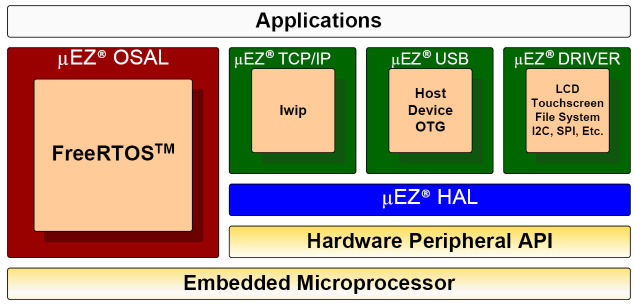
\includegraphics[scale=0.7]{uEZ.png}
\caption{architettura del sistema uEZ}\label{fig:1}
\end{figure}

Il sistema offre innanzitutto un HAL piuttosto potente, in quanto permette di trattare ad alto livello la configurazione di tutte le periferiche. Inoltre non è necessario definire il boot di sistema (cosa non banale per questi sistemi). Esiste un porting standard per ogni processore, se non è presente è possibile scriverlo facilmente. Il sistema deve essere compilato in due passaggi: il primo consiste nel compilare $\mu EZ$ per la propria architettura, ottenendo un file di libreria da linkare al proprio progetto, il secondo consiste nello sviluppare il proprio progetto basandosi su questo sistema. È possibile, al tempo di compilazione, decidere quali periferiche utilizzare prima di generare la libreria da linkare, ottimizzando per area il proprio software.




Ciò che ha portato allo sviluppo su questo sistema software è stato, oltre all'astrazione dell'hardware che facilita la programmazione e alla predisposizione da parte del sistema di usare risorse di rete come lo stack di rete lwIP, è stata la capacità di utilizzare una libreria grafica molto importante e potente per i sistemi embedded, la libreria \textbf{emWIN}.

\subsection{emWin}





\section{Diagramma dei componenti Software}

%%%%%%%%%%%%%%%%%%%%%%%%%%%%%%%%%%%%%%%%%%%%%%%%%%%%%%%%%%%%%%%%%%%%%%%%%%%%%%%%%%%%%%%%%%%%%%%%%%%%%%%%%%%%%%%%%%%%%%%%%%%%%%%%%%%%%%%%%
%%%%%%%%%%%%%%%%%%%%%%%%%%%%%%%%%%%%%%%%%%%%%%%%%%%%%%%%%%%%%%%%%%%%%%%%%%%%%%%%%%%%%%%%%%%%%%%%%%%%%%%%%%%%%%%%%%%%%%%%%%%%%%%%%%%%%%%%%
%%%%%%%%%%%%%%%%%%%%%%%%%%%%%%%%%%%%%%%%%%%%%%%%%%%%%%%%%%%%%%%%%%%%%%%%%%%%%%%%%%%%%%%%%%%%%%%%%%%%%%%%%%%%%%%%%%%%%%%%%%%%%%%%%%%%%%%%%
%%%%%%%%%%%%%%%%%%%%%%%%%%%%%%%%%%%%%%%%%%%%%%%%%%%%%%%%%%%%%%%%%%%%%%%%%%%%%%%%%%%%%%%%%%%%%%%%%%%%%%%%%%%%%%%%%%%%%%%%%%%%%%%%%%%%%%%%%

\chapter{Modello di sistema}

Di seguito si riporta il modello del sistema secondo lo standard ingegneristico, ossia presentando:
\begin{itemize}[noitemsep,topsep=23pt,parsep=23pt,partopsep=0pt]

\item\textit{``Use Case Diagram''}, ossia la presentazione ad alto livello dei diversi attori del sistema (nel nostro caso gli attori sono: l'utente, il dispositivo Master e il dispositivo Slave), in modo da rendere chiari i ruoli degli attori e le loro azioni all'interno dello scenario;
\item\textit{``Sequence Diagram''}, ossia la presentazione ad alto livello dello scambio di ``messaggi'' tra i diversi attori e dispositivi del sistema (vengono identificate le interazioni nel sistema come messaggi);

\end{itemize}

\newpage

\section{Use Case Diagram}

Con questo tipo di diagramma, viene presentata una tabella per ogni attore, ciascuna contenente nell'intestazione il nome dell'attore considerato e all'interno le rispettive azioni. Ogni attore coinvolto nel sistema ha delle precondizioni da rispettare affinchè tutte le operazioni vadano a buon fine e una postcondizione. Vengono presentate infine le azioni sotto forma di algoritmo o insieme di attività da svolgere per eseguire un task.

L'attore principale, cioè l'utente, ha tre tipi di attività, ossia la scelta del task da far eseguire al sistema, l'avvio di esecuzione di tale task (premendo l'opportuno tasto nell'interfaccia) e l'osservazione dei valori che vengono mostrati nella GUI.

L'altro attore è il dispositivo Master, che ha il compito di mostrare ed aggiornare l'interfaccia grafica e di interrogare il dispositivo Slave in base alla scelta dell'utente. Questo attore ha quindi queste attività: mostrare l'interfaccia grafica, avviare i task scelti dall'utente e inviare i messaggi ai dispositivi Slave.

Gli ultimi attori da considerare sono i dispositivi Slave, che hanno il compito di eseguire polling sui sensori a loro associati e di rispondere alle richieste Modbus del dispositivo Master. Le loro attività quindi sono: controllo sensori e ricezione e risposta di messaggi Modbus.

~

~

\begin{usecase}
  \addheading{Attore}{Utente} 
  \addrow{Precondizione}{Il sistema è avviato e mostra la GUI a seguito del logo $\mu EZ$, tutti i tasti sono selezionabili e tutti i dispositivi sono avviati.}
  \addrow{Postcondizione}{L'utente è munito di penna specifica per interfacciarsi col dispositivo TouchScreen.}
  \addmulrow{Scelta task}	{\item interfaccia gestione LED
                             	\item interfaccia monitoraggio sensori
				\item interfaccia di debug}

  \addmulrow{Esecuzione task}	{\item accendere o spegnere luci
                             	\item controllo sensori
				\item attività di debug}

  \addmulrow{Osserva valori}	{\item valutazione valori mostrati dalla GUI}

\end{usecase}

\begin{usecase}

  \addheading{Attore}{Master} 
  \addrow{Precondizione}{Il sistema è avviato.}
  \addrow{Postcondizione}{L'utente esegue scelte.}
  \addmulrow{Mostra GUI}	{\item mostra schermata principale}

  \addmulrow{Avvia task}	{\item ottieni scelta dall'utente}

  \addmulrow{Invia messaggi}	{\item messaggi di tipo read
				\item messaggi di tipo write}
  

\end{usecase}


\begin{usecase}

  \addheading{Attore}{Slave} 
  \addrow{Precondizione}{Il sistema è avviato.}
  \addrow{Postcondizione}{I sensori rispondono e si ricevono correttamente messaggi Modbus.}
	\addmulrow{Controllo}	{\item esegue polling sui sensori
				\item aggiorna il valore dei registri col valore ottenuto dai sensori}
  \addmulrow{Ricezione}		{\item riceve messaggi Modbus
				\item invia o setta i registri richiesti }

\end{usecase}


\newpage

\section{Sequence Diagram}

Questo diagramma rappresenta una generica interazione tra utente e sistema. Ad ogni scelta dell'utente, visualizzabile come un messaggio (ovviamente non testuale) inviato dall'utente al dispositivo Master, viene trasformata in messaggio Modbus da inviare al corrispondente dispositivo Slave. Il dispositivo Slave, prima di essere interrogato via Modbus, continua ad eseguire polling sui sensori a lui collegati, per tenersi aggiornato sul loro valore. Al momento della richiesta Modbus, il disposivo Slave termina momentaneamente di eseguire polling sui sensori e invia l'ultimo valore acquisito da questi al dispositivo Master. Quest'ultimo, appena riceve i valori, aggiorna l'interfaccia grafica e mostra all'utente il risultato dell'interrogazione. Fatto ciò, il dispositivo Master rimane in attesa di ordini dall'utente, mentre il dispositivo Slave continua a fare polling sui sensori a lui collegati.

~

\begin{figure}[!hb]
  \centering
  \begin{sequencediagram}

    \newthread{ut}{:Utente}	%rettangolo sempre attivo
    \newinst[2.5]{ms}{:Master}		%solo tratteggiato
    \newinst[2.5]{sl}{:Slave}

        \begin{callself}{sl}{PollSensori()}{}
        \end{callself}
        \begin{callself}{sl}{PollSensori()}{}
        \end{callself}
        \begin{callself}{sl}{PollSensori()}{}
        \end{callself}
    
      	\begin{call}{ut}{EseguiScelta()}{ms}{}

		\begin{call}{ms}{inviaRichiestaModbus()}{sl}{}
		\end{call}

		\begin{callself}{ms}{aggiornaGUI()}{}
		\end{callself}



      	\end{call}

		\begin{callself}{sl}{PollSensori()}{}
		\end{callself}
		\begin{callself}{sl}{PollSensori()}{}
		\end{callself}
		\begin{callself}{sl}{PollSensori()}{}
		\end{callself}


  \end{sequencediagram}
  \caption{Esempio di attività generica con il sistema.}
\end{figure}


\newpage






\end{document}
\endinput
